\documentclass[]{article}
\usepackage{amsmath,amsfonts,amssymb,amsthm}
\usepackage{hyperref}
\usepackage[all]{xy}
\usepackage{fullpage}
\usepackage{hyperref}
\usepackage{color}
\usepackage{graphicx}
\newcommand{\taylor}[1]{{\color{blue} \sf $\spadesuit\spadesuit\spadesuit$ Taylor: [#1]}}
%\newcommand{\collab}[1]{{\color{red} \sf $\spadesuit\spadesuit\spadesuit$ collab1: [#1]}}  %Dear Collaborator, make a macro for yourself here. 
\newcommand{\todo}[1]{{\color{purple} \sf $\spadesuit\spadesuit\spadesuit$ TODO: [#1]}}

\numberwithin{equation}{section}
\newtheorem{theorem}{Theorem}[subsection]
\newtheorem{lemma}[theorem]{Lemma}
\newtheorem{corollary}[theorem]{Corollary}
\newtheorem{proposition}[theorem]{Proposition}

\theoremstyle{definition}
\newtheorem{definition}[theorem]{Definition}
\newtheorem{question}[theorem]{Question}
\newtheorem{conjecture}[theorem]{Conjecture}
\newtheorem{example}[theorem]{Example}
\newtheorem{exercise}[theorem]{Exercise}

\theoremstyle{remark}
\newtheorem{remark}[theorem]{Remark}
\newtheorem{remarks}[theorem]{Remarks}
\newtheorem{warning}[theorem]{Warning}


%opening



\begin{document}
	
\begin{center}
	{\Large \sc Dupuy -- Math 1077  --Reflections }\\
	last updated: \today
\end{center}

\noindent This document contains all of the reflection questions for Math 1077. 
There are no right or wrong answers to these questions. They are intended to get you thinking about a certain topic before we engage with them in class.
\vspace{1em}

\noindent {\bf WARNING}: Prior to their being assigned a due date reflection questions are subject to change! This includes, but is not limited, to the order in which reflection questions are given and title of the reflections. Some of the reflections might not be assigned at all!

\tableofcontents

\newpage

\subsection{Calculators and Really Small Numbers }
We often take calculators for granted. 
\begin{enumerate}
\item Find you nearest calculator (google, iPhone, or laptop will work) and input $31+10^{-16}$. That is, try to get it to perform the addition 
$$31 + 0.0000000000000001.$$
\item  What computer did you use? What happened? 
\item Try it on another system. (If you didn't find something weird, try it on Google (as of Fall 2023 this works); you can also try increasing 16 to 32.)
\item Why do you think this happens?
\item What is the largest number such that 1 plus that number returns 1 on that device?  (Usually it is $10^{-16}$. For fancier computers it is $10^{-32}$. For very fancy computers it would be $10^{-64}$.)
\end{enumerate}



\subsection{Expected Values Are Everywhere }
Expected values are everywhere.
They can be used in games, psychology experiments, interpersonal relationships, business, biology, and elsewhere. 
\begin{enumerate}
	\item What is the ``expected value'' of a random event? (Give you best mathematical definition)
	\item Give an example of an expected value that you care about? This can be from a game you play or from something you like to collect or anything really. 
\end{enumerate}

\subsection{Bernoulli's Game}\footnote{Ellenberg ``St Petersburg and Ellsburg'' pg 242}
Consider the following five dollar carnival game. 
In this game, you are asked to repeatedly toss a coin and the game stops the first time you flip heads. 
The payout structure is as follows:
\begin{itemize}
	\item if you flip heads (H) your first try you get \$1. 
	\item if you flip tails then heads (TH) you get \$2.
	\item if you flip two tails then a heads (TTH) you get \$4. 
	\item if you flip TTTH you get \$8.
	\item $\cdots$
\end{itemize}	
The pattern keeps going with the payout doubling for each tail you flip in a row. 
\begin{enumerate}
\item Should you play this game?
\item How much should you pay to play this game?
\end{enumerate}

\subsection{Flipping Coins }
Produce a sheet of paper with 200 coin flips recording a sequential number of heads and tails. There are two ways you can do this. 
You can cheat and just write down a bunch of heads and tails or you actually flip a coin 200 times. 
All I ask is that you don't mix these two ways of completing this assignment.
Either completely cheat and just write down random heads and tails or you actually flip coins and do this for the entire 200 flips.
When you submit the assignment don't say which method you used.

\subsection{$p$-values}	
Consider the xkcd comic at the following link:
\begin{center}
	\url{https://xkcd.com/882/}.
\end{center}
What do you think this comic is making fun of?


\subsection{Repeating Events}
\begin{enumerate}
	\item Suppose you are going to buy a lottery tickey and the only prize is the jackpot. In the game you select six numbers 1-50. Which ticket is better?: 
	$$\mbox{ticket one:} \quad  1,1,1,1,1,1. $$
	$$\mbox{ticket two:} \quad 12,26,3,50,24,27.$$
	Why?
\item Suppose you are flipping a coin and you flip 10 heads in a row. Is it more likely that you flip a tails the next time?
\item You flip 5 coins. Which outcome is more likely HHHHH or HTHTH?
\end{enumerate}

\subsection{The Monty Hall Problem } 
You are the contestant an \emph{Let's Make A Deal} with host Monty Hall! In this game there are three doors. Behind two of the doors there are goats and behind one of the doors is a brand new car. Your job is to guess which door has the car and if you get it right, you get the car. Monty asks you to select a door. After your selection he reveals goats behind one of the doors. You are allowed to stay with your current door or switch. 
\begin{enumerate}
\item What should you do? Should you stay with your current door? Should you switch to the new door? 
\item Does it matter? Explain your answer.
\end{enumerate}

\subsection{What is Ranked Choice Voting? }
In 2009 Burlington had an election for Mayor in which there were three candidates. At the time the city implemented ``ranked choice voting" which is a system in which voters submit a ballot which ranks their perferred order of candidates. 

\begin{enumerate}
	\item How do you suppose this worked? Make up some rules that would allow you to elect a mayor to take into account the voters will using these ranked ballots. 
	\item If you were allowed to make up a voting system how would it work? (Make up a ranked choice voting system and explain your rules.) 
	\item Why?
\end{enumerate}
	
	\newpage
\subsection{Seven Bridges of Koenigsburg }
Euler lived in the city of \href{https://goo.gl/maps/h28p2rEpXZGGkn9M6}{Koenigsberg} (modern day Kaliningrad). The city had a system of bridges as mapped out below in Figure~\ref{F:seven-bridges}. 
\begin{figure}[htbp!]
	\begin{center}
		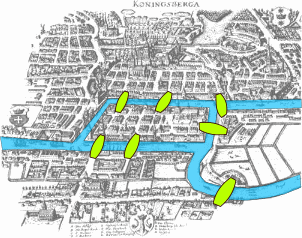
\includegraphics[scale=0.5]{konigsberg_bridges.png}
	\end{center}
	\caption{The city of Koenigsburg and its seven bridges.}\label{F:seven-bridges}
\end{figure}
Euler wanted to find a route through the city to walk across each one of the bridges exactly once in the city. 
\begin{enumerate}
\item How can Euler achieve such a route? 
\item Make a map and try making a route that achieves this. 
\end{enumerate}


	
\subsection{The Three Houses and Three Utlilities Puzzle}
	My 5th grade teacher math Mrs. Kelly gave me the following problem in 1995: 
	\begin{figure}[htbp!]
		\begin{center}
			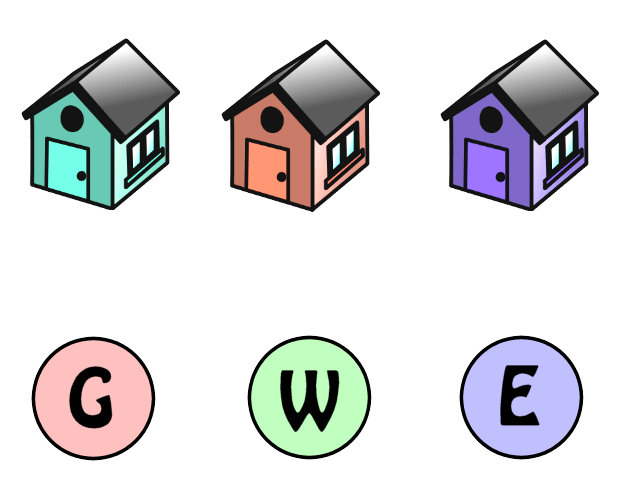
\includegraphics[scale=0.25]{three-houses.png}
		\end{center}
		\caption{A image of the three houses and three utilities problem.  Image taken from \href{http://puzzles.nigelcoldwell.co.uk/twentysix.htm}{Nigel Coldwell's webpage.} }
	\end{figure}
	There are three houses and three utilities as pictured below.
	Each how needs water, electric, and gas, but the water line, electric line, and gas line are not allowed to cross each other (pretend that the construction workers will explode or something if this happens).
	\begin{enumerate}
	\item Draw a line connecting each of the three houses to each of the three utilities without any of the lines cross each other. 
	\item What do you observe?
	\end{enumerate}
	
\subsection{The Prisoner Puzzle }

An evil Warden is going to play a game with his prisoners for their freedom. 
He tells them that he has hidden all of their inmate numbers in boxes in the dining hall. Each prinsoner is given a chance to enter a room and find their number which is hidden in one of the boxes and they are allowed to open 25 boxes.
After each prinsoner leaves the dining hall, the numbers are reset. 
If \emph{all} of the prisoners find their number they will all be set free.

\noindent Here are the questions:
\begin{enumerate}
\item What does it seem like the probability of success will be for the prisoners?
\item What strategy should the prisoners use to maximize their chances of escape? (Spoiler: there exists a strategy that works about 30\% of the time).
\end{enumerate}

\noindent Here are the technical parts of the puzzle:

\begin{itemize}
	\item There are 50 prisoners numbered 1--50.
	\item There are 50 boxes numbered 1--50 in the room.
	\item Each of the numbers 1--50 are placed in the boxes at random. 
	\item Each number appears in a box exactly once. (So for example the number 7 could be placed in box 20, but it won't be in any other boxes. We are also guaranteed that the number 7 will appear in some box.)
	\item Each prisoner is allowed to open 25 boxes of their choosing.
	\item After a prisoner leaves the room, the boxes and numbers are reset to their original configuration. (So all of the prisoners get the same setup every time they enter the room).
	\item The prisoners are allowed to communicate before the game starts but are not allowed to communicate after the game has started. 
	\item There is no way for the prisoners to share information after the game starts.
\end{itemize} 


\iffalse 
\subsection{}	
	\taylor{TBD $p$-value}
	
\subsection{}
	
	\taylor{TBD regression to the mean}
	
\subsection{M\"obius Band}
What do you think will happen if we take a M\"obius band and cut it down the middle?

\fi 
%\bibliographystyle{amsalpha}
%\bibliography{mydocument.bib}

\end{document}
